%% bare_conf.tex
%% Midterm progress report

\documentclass[conference,a4paper]{IEEEtran}

% --- Packages ---
\usepackage{graphicx}
\usepackage{booktabs}
\usepackage{amsmath}
\usepackage{tikz}
\usepackage{pgfplots}
\pgfplotsset{compat=1.18}

% --- Hyphenation ---
\hyphenation{op-tical net-works semi-conduc-tor RISC-V}

% --- Author footnote helper ---
\DeclareRobustCommand*{\IEEEauthorrefmark}[1]{\raisebox{0pt}[0pt][0pt]{\textsuperscript{\footnotesize #1}}}

\begin{document}

\title{Hint-Based VLIW Extensions for the RISC-V Wally Core:\\
Midterm Progress Toward Floating-Point Parallelism}

\author{\IEEEauthorblockN{
Leo Marek\IEEEauthorrefmark{1},
Gregory Chekler\IEEEauthorrefmark{1}*,
Jing Jing Chen\IEEEauthorrefmark{1}*,
Elliot Chae\IEEEauthorrefmark{1}*,\\
Ethan Carr\IEEEauthorrefmark{1}* and
Ray Simar\IEEEauthorrefmark{1}
}
\IEEEauthorblockA{\IEEEauthorrefmark{1}Department of Electrical and Computer Engineering, Rice University, Houston, USA\\
Email: \{lnm7, gsc8, jc165, ejc12, ehc6, ray.simar\}@rice.edu}
\IEEEauthorblockA{*Equal Contribution}
}

\maketitle

\begin{abstract}
Very Long Instruction Word (VLIW) architectures expose instruction-level parallelism through static scheduling, avoiding much of the control complexity required by superscalar execution. This project explores a hint-based VLIW extension to RISC-V implemented on the OpenHW Group CVW (Wally) core. Architecturally reserved HINT instructions encode bundle information while remaining compatible with standard binaries. 

This report describes midterm progress toward a semester goal of enabling floating-point parallelism on Wally. The current effort centers on completing an integer VLIW implementation and validating it in simulation before extending the design further. The integer execution path now supports bundled issue and has been checked against scalar behavior. In parallel, work has begun on a floating-point register file and on evaluating how many execution lanes should support floating-point operations. Preliminary experiments on DSP-style kernels provide an initial baseline for future floating-point studies and help frame the remaining architectural tradeoffs.
\end{abstract}

{\smallskip \keywords RISC-V, VLIW, Wally, floating point, DSP, instruction-level parallelism, MPACT.}

\section{Introduction}

Embedded processors must balance performance, power, and implementation complexity. Superscalar processors can extract substantial instruction-level parallelism (ILP), but doing so requires dynamic scheduling, hazard detection, operand tracking, and often speculation. These features can improve performance, but they also increase hardware cost and design complexity. VLIW architectures take a different approach by exposing ILP through static scheduling, moving more of the burden to software while keeping the hardware simpler.

This project explores a hybrid design in which reserved RISC-V HINT instructions encode VLIW bundle information. On an unmodified RISC-V implementation, these instructions behave as no-ops, preserving compatibility with standard binaries. On a modified Wally core, however, the same instructions indicate that the following instructions may be issued in parallel. This allows parallel issue without introducing the full machinery of a conventional superscalar design.

The long-term goal is to extend this mechanism from integer execution to floating-point workloads. That extension is especially relevant for DSP-style kernels and other structured workloads where multiple arithmetic operations can often be scheduled together. The main objectives for the semester are:

\begin{itemize}
    \item implement integer VLIW execution and verify that it matches scalar results in RTL simulation,
    \item design and implement a floating-point register file,
    \item evaluate how many execution lanes should support floating-point operations, and
    \item establish a path toward compiling floating-point workloads using the MPACT simulator.
\end{itemize}

At this point, the integer VLIW design is the most mature component of the project and serves as the basis for the floating-point extension. The floating-point work is still earlier in development, but the core implementation questions and evaluation framework are now taking shape.

\section{Methods}

\subsection{Architectural Approach}

The architecture uses RISC-V HINT instructions to communicate static scheduling decisions to a modified Wally pipeline. A HINT instruction specifies the size of a bundle, and the subsequent instructions are treated as a parallel group when the architectural constraints for bundled issue are satisfied. This preserves the meaning of the original instruction stream while allowing the hardware to exploit additional ILP when the code has been scheduled appropriately.

The current implementation targets a four-lane issue structure. Early development therefore focused on the integer datapaths, bundle dispatch logic, and a register file capable of supporting multiple simultaneous reads and writes. This phase was important because integer execution provides a simpler environment in which to test bundle semantics before introducing the additional complexity of floating-point units and floating-point state.

\subsection{ISA Modeling in MPACT}

The initial design was modeled in the Google MPACT simulator. This provided a fast environment for validating bundle semantics, instruction decoding, and execution behavior before making RTL changes. MPACT also made it easier to reason about expected scheduling opportunities and to check that the HINT-based encoding behaved consistently across representative kernels.

In addition to validating the integer design, the simulator is expected to play a central role in the floating-point phase of the project. The current software plan is to target MPACT first with compiler-generated floating-point VLIW code before attempting full hardware integration. In that sense, MPACT serves both as a prototyping platform and as a bridge between ISA experimentation and RTL implementation.

\subsection{RTL Implementation}

The OpenHW Group CVW (Wally) core serves as the RTL baseline. Fetch and decode logic were extended to recognize the HINT-based bundle format and dispatch instructions across multiple execution lanes. Supporting four-lane integer issue required expanding the register file and updating datapath routing so that multiple operations could make progress in the same cycle.

The work so far has emphasized integer execution because it is the clearest intermediate milestone for the semester. Before moving to floating-point functionality, the project must show that the integer version can run bundled code correctly and produce results matching the scalar baseline. Establishing that correctness is essential, since the floating-point design will build directly on the same bundle and dispatch structure.

\subsection{Floating-Point Extension}

The floating-point extension introduces three major changes:

\begin{enumerate}
    \item a dedicated floating-point register file,
    \item additional decode and datapath routing for floating-point instructions, and
    \item an evaluation of how many execution lanes should support floating-point units.
\end{enumerate}

A key design question is whether every lane should support floating-point execution. Full support maximizes peak throughput, but it also increases hardware cost and may leave some resources underused if benchmark behavior does not provide enough parallel floating-point work. A smaller number of floating-point lanes may offer a better balance if performance gains flatten after one or two units. For that reason, the lane-allocation question is being treated as a quantitative design decision rather than as a fixed architectural assumption.

\subsection{Benchmark Strategy}

The current benchmark suite includes handwritten implementations of dot product, FIR, and FFT kernels. These workloads contain substantial instruction-level parallelism and provide useful early tests for the integer execution paths. They also make it easier to inspect the effect of scheduling decisions because their dataflow is relatively structured and their arithmetic behavior is well understood.

Future work will extend this suite with floating-point kernels such as floating-point dot product and IIR filters. The project may also examine additional structured arithmetic workloads that are simple enough to schedule carefully but still representative of common DSP behavior. Longer term, the goal is to move beyond handwritten assembly and compile at least one floating-point workload automatically using a modified LLVM-based toolchain. Reaching that point would demonstrate not only that the hardware can support the design, but also that there is a practical software path for targeting it.

\section{Results}

\subsection{Current Status}

At the midpoint of the semester, the integer portion of the design is functional in simulation and provides a baseline for further experimentation. Progress toward the main objectives is summarized below:

\begin{itemize}
    \item \textbf{Integer VLIW implementation:} bundled execution working in simulation.
    \item \textbf{RTL correctness validation:} ongoing comparison against scalar execution.
    \item \textbf{Floating-point register file:} currently under design.
    \item \textbf{Floating-point lane allocation:} evaluation framework defined.
    \item \textbf{Compiler support:} early exploration using MPACT.
\end{itemize}

Taken together, these results show that the project has moved beyond the planning stage for integer execution and now has a concrete baseline from which performance and architectural tradeoffs can be studied. At the same time, the floating-point portion remains a forward-looking part of the report, with the current work focused on setting up the right implementation and evaluation framework.

\subsection{Integer Benchmark Behavior}

Initial benchmarks focus on DSP-style kernels that expose meaningful instruction-level parallelism. The results shown here use placeholder values and will be replaced with measured data from simulation or hardware experiments. Even so, the figure illustrates the kind of comparison that will matter most in the final report: whether bundled execution provides a worthwhile speedup while preserving correctness.

\begin{figure}[h]
\centering
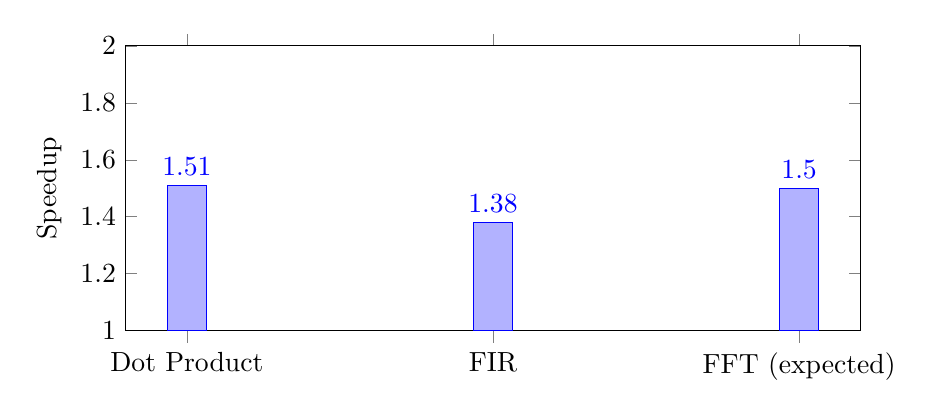
\begin{tikzpicture}
\begin{axis}[
    ybar,
    bar width=14pt,
    width=0.90\linewidth,
    height=5.2cm,
    ylabel={Speedup},
    symbolic x coords={Dot Product,FIR,FFT (expected)},
    xtick=data,
    ymin=1,
    ymax=2,
    nodes near coords,
    nodes near coords align={vertical}
]
\addplot coordinates {(Dot Product,1.51) (FIR,1.38) (FFT (expected),1.5)};
\end{axis}
\end{tikzpicture}
\caption{Preliminary speedup of the integer VLIW implementation over scalar execution.}
\label{fig:speedup}
\end{figure}

Although the values in Figure~\ref{fig:speedup} are placeholders, the figure captures the central performance question for the integer design. If the measured speedups remain meaningful after full validation, then the project will have met an important milestone toward establishing the usefulness of the hint-based VLIW approach.

\subsection{Floating-Point Lane Exploration}

Determining how many lanes should support floating-point operations is a central design question for the second half of the project. Figure~\ref{fig:fp_lane_scaling} illustrates the type of analysis that will guide this decision. The goal is not simply to maximize throughput, but to understand where additional floating-point hardware stops producing worthwhile gains.

\begin{figure}[h]
\centering
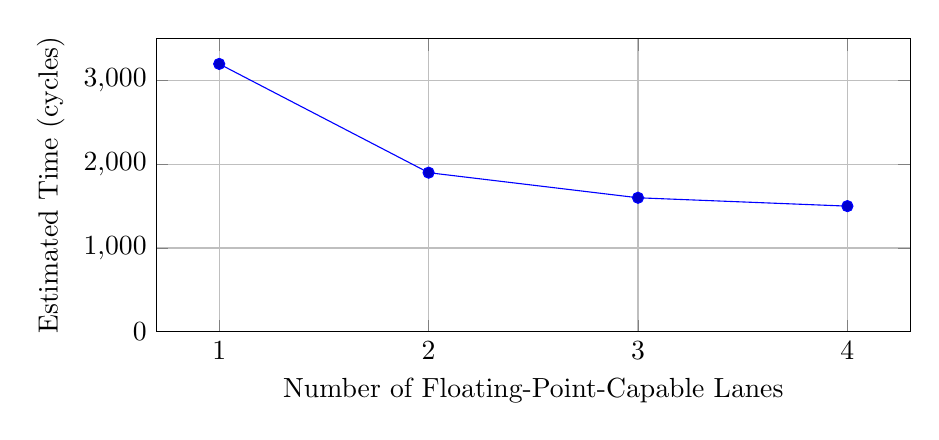
\begin{tikzpicture}
\begin{axis}[
    width=0.92\linewidth,
    height=5.3cm,
    xlabel={Number of Floating-Point-Capable Lanes},
    ylabel={Estimated Time (cycles)},
    xtick={1,2,3,4},
    xmin=0.7,
    xmax=4.3,
    ymin=0,
    ymax=3500,
    mark=*,
    grid=both
]
\addplot coordinates {(1,3200) (2,1900) (3,1600) (4,1500)};
\end{axis}
\end{tikzpicture}
\caption{Expected performance effect of increasing the number of floating-point lanes.}
\label{fig:fp_lane_scaling}
\end{figure}

If future measurements show that performance improves sharply when moving from one floating-point lane to two, but only marginally beyond that, then a partially floating-point-capable architecture may be a better tradeoff than full replication across all lanes. That question will become more concrete once the floating-point datapath and benchmark support are in place.

\section{Discussion}

The integer VLIW implementation now provides a working proof of concept for the hint-based approach on the Wally core. The design shows that bundled execution can be introduced while preserving compatibility with the base RISC-V ISA, which is one of the more attractive aspects of the overall approach. Rather than defining an entirely separate execution model, the project layers static scheduling information onto existing instructions in a way that remains safe on an unmodified core.

The next step is to complete validation of the integer pipeline and replace placeholder results with measured data. That includes confirming scalar-equivalent behavior in RTL and quantifying the performance benefit of bundled issue across the benchmark suite. These measurements will determine whether the current design provides enough benefit to justify the added implementation complexity.

Once the integer design is stable, the floating-point extension will become the primary focus. That phase involves more than attaching floating-point units to the existing lanes. It also requires a floating-point register file, additional decode and routing support, and a careful decision about how widely floating-point capability should be distributed. Those choices affect both performance and implementation cost, so they need to be justified with actual benchmark data rather than intuition.

Software support remains another major challenge. Handwritten assembly has been useful for early testing and controlled experiments, but it is not a practical long-term interface. A meaningful milestone for the second half of the semester is therefore to demonstrate that at least one floating-point kernel can be compiled into a bundled form and executed correctly on MPACT. Reaching that point would strengthen the argument that the architecture is not just an interesting RTL exercise, but something that can also be targeted by a realistic tool flow.

Overall, the project has reached a useful midterm point: the integer path is concrete enough to validate and measure, while the floating-point work is now defined clearly enough to guide the next stage of implementation. That makes the remaining work more focused than exploratory and gives the project a clear direction for the rest of the semester.

\section*{Acknowledgment}

The authors thank David Harris and the OpenHW Group for the open-source CVW core and the developers of the Google MPACT simulator for providing a flexible platform for architectural experimentation. AI coding assistants including Gemini, Claude, and Codex were used to help with code generation, debugging, and documentation.

\section*{CRediT Author Statement}

Leo Marek: Conceptualization, Methodology, Software, Validation, Formal Analysis, Investigation, Visualization, Writing -- Original Draft, Writing -- Review \& Editing. Gregory Chekler: Methodology, Validation, Investigation, Writing -- Review \& Editing. Jing Jing Chen: Methodology, Validation, Investigation, Writing -- Review \& Editing. Elliot Chae: Methodology, Validation, Investigation, Writing -- Review \& Editing. Ethan Carr: Methodology, Validation, Investigation, Writing -- Review \& Editing. Ray Simar: Conceptualization, Supervision, Resources.

\begin{thebibliography}{9}

\bibitem{RISCV-Spec}
A.~Waterman and K.~Asanovi\'{c},
\emph{The RISC-V Instruction Set Manual, Volume I: User-Level ISA}.

\bibitem{Wally}
D.~Harris et al.,
\emph{The RISC-V Wally Processor}.

\bibitem{MPACT}
Google,
\emph{MPACT Simulator Framework}.

\end{thebibliography}

\end{document}